\section{Mathematical model}\label{sec:MathModel}
A simplified model of a quadruped robot, depicted in Fig. \ref{fig:rmoment} has three distinctive parts: the main body, the tail and four legs. Let the frame $L$ be defined with its origin $\vec{O}$ and the respective coordinate system, then the following key frames should be observed: $L_w$ - world frame, $L_c$ - geometrical center of construction frame; $L_B$ - main body's center of mass frame; $L_T$ - tail's center of mass frame; and $L_{pi}$ - $i$-th leg point of contact frame. The proposed mathematical model is derived under the assumption of a stable locomotion maneuver which includes vertical (jumping) and horizontal movement of the robot. For such a maneuver, the legs need to develop periodic horizontal and vertical forces denoted as side force $\textbf{S}_{pi}$ and thrust force $\textbf{T}_{pi}$ respectively. In order to achieve these forces, an adequate leg joint trajectory needs to be planned. Trajectory planning for the leg joints goes beyond the scope of this paper. 

\begin{figure}
	\centering
	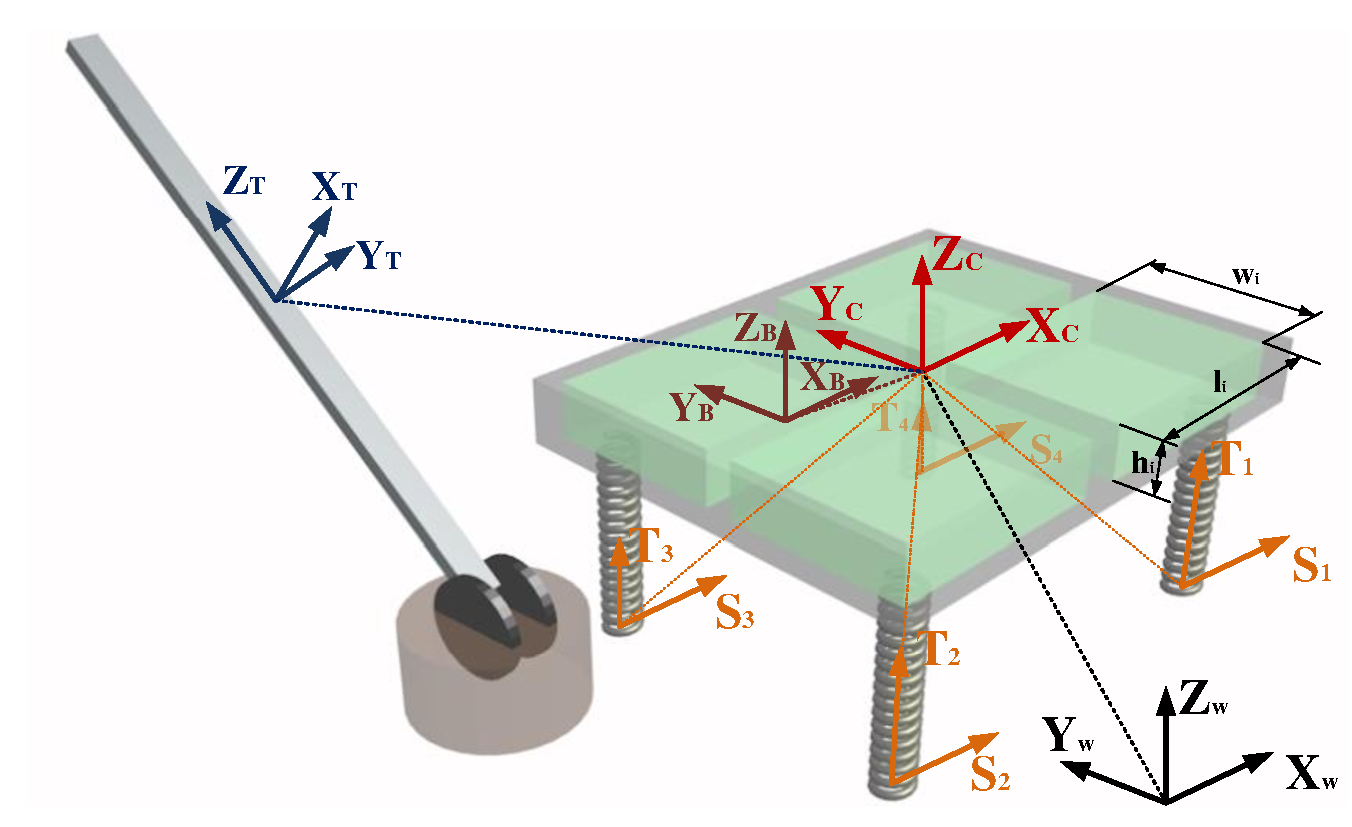
\includegraphics[width=85mm]{./pictures/RobinMoment.pdf}
	\caption{Robin body dynamics}
	\label{fig:rmoment}
\end{figure}

\subsection{Main body dynamics}
In order to simplify the complexity of the analysis, quadruped's main body is modeled as a system of four, equally displaced cuboid shaped bodies, as shown in Fig \ref{fig:rmoment}. Ideally, when the robots's body is fully symmetric, all four cuboids have the same mass. Since, in most situations, this is not the case, each cuboid has its own mass $m_i$, with its own centroid $\vec{\textbf{cm}}_i$. Each cuboid element center of mass $\vec{\textbf{cm}}_i$ is then placed at $\vec{\textbf{r}}_i$ distance from the body geometric center, the $L_c$ coordinate system. The overall main body center of mass is then easily calculated with:
 
\begin{equation}\label{eq:CMrobot}
\vec{\textbf{r}_{CM}}=\frac{\sum_{i=1}^{4}m_i\vec{\textbf{r}}_i}{\sum_{i=1}^{4}m_i}
\end{equation}

Vector $\vec{\textbf{r}_{CM}}$ points from the center of construction frame $L_C$ to the center of mass frame $L_B$, quantifying the displacement of the center of mass from the construction center of the robot. Next important dynamic parameter is the tensor of inertia. Having four prismatic bodies as the basis for the robot model, tensor of inertia can easily be derived using the Parallel axis theorem:

\begin{equation}
\footnotesize
\textbf{J}_R=\sum_{i=1}^{4}\left \{\textbf{J}_{c_i}+m_i\begin{bmatrix}
{_yr_i}^2+{_zr_i}^2 & {_xr_i}\cdot {_yr_i} & {_xr_i}\cdot {_zr_i} \\ 
-{_xr_i}\cdot {_yr_i} & {_xr_i}^2+{_zr_i}^2 & {_yr_i}\cdot {_zr_i}\\ 
-{_xr_i}\cdot {_zr_i} & {_yr_i}\cdot {_zr_i} & {_yr_i}^2+{_xr_i}^2
\end{bmatrix} \right \}
\normalsize
\end{equation}

where, $_xr_i, _yr_i, _zr_i$ represent the $x,y,z$ projection of $\vec{\textbf{r}}_i$, and $\textbf{J}_{c_i}$ is the tensor of inertia of a single cuboid of height $h_i$, width $w_i$ and depth $d_i$ as indicated in Fig. \ref{fig:rmoment}:
\begin{equation}
\textbf{J}_{c_i}=\frac{m_i}{3}\begin{bmatrix}
w_i^2+d_i^2 &0&0 \\ 
0 &h_i^2+d_i^2&0\\ 
0 &0& w_i^2+h_i^2
\end{bmatrix}
\end{equation} 

It could be easily shown that if all four body parts have the same mass and size (i.e. $m,h,d,w$) in addition to lying symmetrically displaced around the body center frame $L_c$, as depicted in Fig \ref{fig:rmoment}, the total body moment of inertia $J_R$ is reduced to a diagonal matrix,
\begin{equation}
\textbf{J}_{R}=\frac{m}{12}\begin{bmatrix}
(2w)^2+d^2 &0&0 \\ 
0 &(2h)^2+d^2&0\\ 
0 &0& (2w)^2+(2h)^2
\end{bmatrix}
\end{equation} 
and the body center of mass is placed directly in the center of the body coordinate system. For any other arrangement, tensor matrix will not be diagonal, and what is even worse, the body center of mass will be misaligned, which in turn, produces undesired in-air rotations.

\subsection{Leg dynamics}
%%%%%%%%%%%%%%%%%%%%%%%%%%%%%%%%%%%%%%%
% Dynarobin,Single leg model 

%\section{Dynarobin leg model}

%This paper goal is to improove locomotion stability on quadrupedal robot Dynarobin, depicted in Fig. \ref{fig:Dynarobin}. 
The robot has four identical legs ($l\in \left \{ 1,2,3,4 \right \}$), each combining three rotational joints: hip, knee, and ankle, respectively. Fig. \ref{fig:DynarobinLEG} depicts one such leg, with each joint marked with a red circle and an additional mechanical spring end-effector. In order to mimic the spring-mass system, each joint controller implements impedance control \cite{citeulike:2203614}. The actual implementation goes beyond the scope of this paper and will not be further discussed. Together with adequate joint trajectory planning and inverse kinematics the legs can be tuned to mimic the behavior of an active spring-mass system \cite{conf/iros/ParkP12}\cite{6171868}, so that when the legs are in the contact with the ground, side forces and thrust forces are produced.

Besides the kinematic chain performing as an active spring, each leg contains an additional mechanical spring that changes the stiffness of the contact with the surface. Combining these mechanical springs together with leg's compliant dynamics enables us to model each leg of the robot as a single, active spring. The simplified quadruped's leg model is shown in Fig. \ref{fig:DynarobinLEG}. It consists of three masses connected by virtual active and passive springs. The passive spring has initial fixed length $L_{pl}=L_{p0}$ and parameters $K_{pl}$ and $C_{pl}$.  The actuated spring has variable parameters $K_{al}$ and $C_{al}$ and actuation is provided by changing the initial length $L_{al}=L_{a0}$ by $\Delta L$.
\begin{figure}[t!]
	\centering
	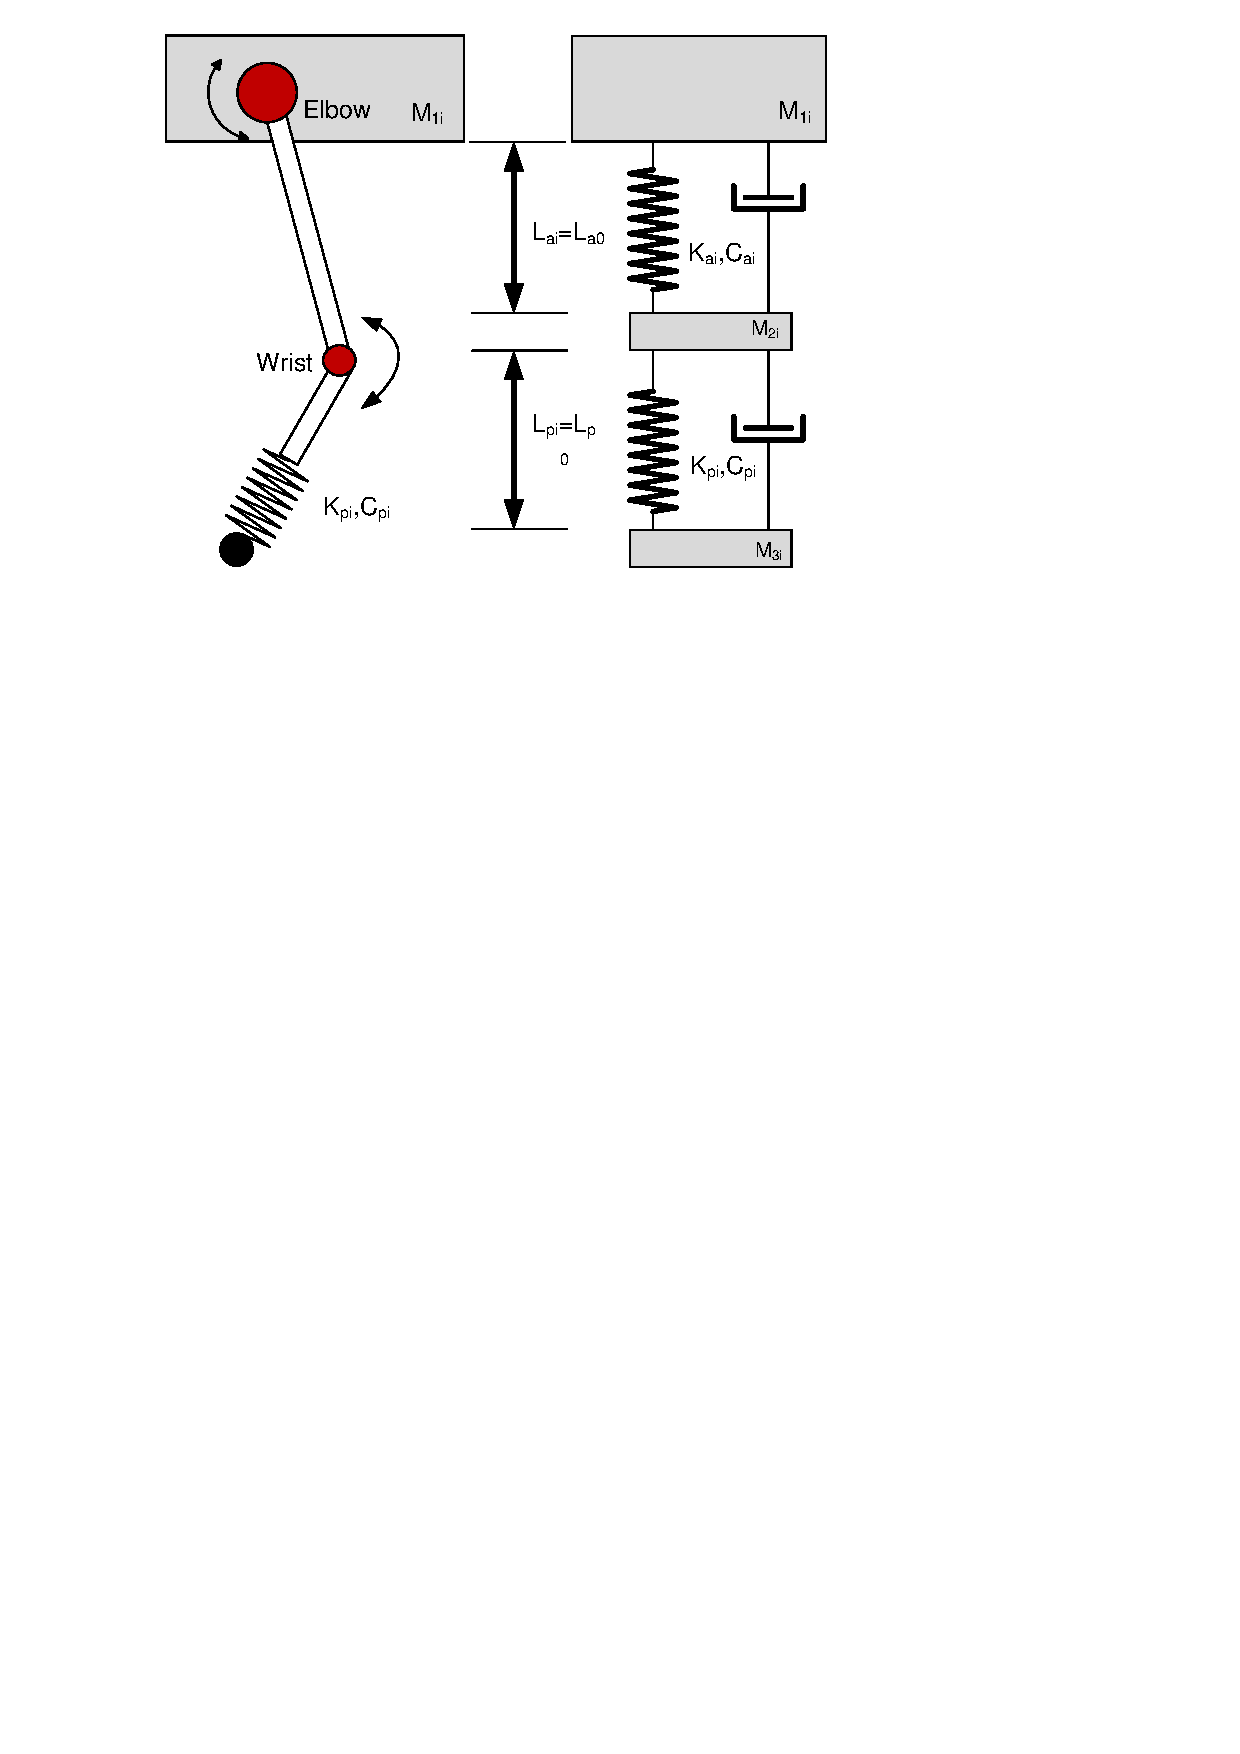
\includegraphics[width=80mm]{./pictures/Dynarobin_leg.pdf}
	\caption{Double spring-mass model of the leg}
	\label{fig:DynarobinLEG}
\end{figure}


%As it was previously explained, we propose modeling quadruped's legs as active springs. This can be achieved through adequat leg joint path planning, so that when the legs are in the contact with the ground, side forces and thrust forces are produced. 
Positioned symmetrically around the geometric center the legs exert forces and torques on the quadruped main body according to:

\begin{gather}\label{eq:Forces}
\vec{\textbf{F}_{tot}}=\sum_{i=1}^{4}(\vec{\textbf{T}_{i}}+\vec{\textbf{S}_{i}})\\
\vec{\boldsymbol{\tau}_{tot}}=\sum_{i=1}^{4}\vec{\boldsymbol{\rho} _i}\times(\vec{\textbf{T}_{i}}+\vec{\textbf{S}_{i}})
\end{gather}  
where $\vec{\textbf{T}_{i}}$ represents the $i$-th body part thrust force that causes vertical movement (i.e. hopping), $\vec{\textbf{S}_{i}}$ $i$-th cuboid 


side force that moves the quadruped in x direction, and $\vec{\boldsymbol{\rho}} _i$ denotes the $i$-th distance between the center mass and 
the origin of forces ($\vec{\boldsymbol{\rho}} _i=\vec{\textbf{r}} _CM+\vec{\textbf{r}} _i$). In reality, one would have the y - component of
the side force, but since this component is of the order of magnitude smaller then the x - component, it can be disregarded.

For a perfectly symmetric body it follows that the total torque (\ref{eq:Forces}) acting on the body is equal to zero, and the total force is the sum of all 4 active springs. For this, the necessary condition is that all four springs have exactly the same parameters (i.e. force magnitudes, distance from the geometric center, etc.), and thus exert the same forces. In reality, neither the springs are the same, nor can there be a perfectly symmetric body. We write the body torque equation for a non-symmetric body, with the center of mass displaced for $\vec{\Delta\textbf{r}_{CM}}$:

\begin{equation}\label{eq:Torques}
\vec{\boldsymbol{\tau}}_{tot}=\begin{bmatrix}
\Delta \textsc{y}_{CM} \:\bar{T} & -\left ( \Delta \textsc{x}_{CM} \:\bar{T} +\Delta \textsc{z}_{CM} \:\bar{S}\right ) & -\Delta \textsc{y}_{CM} \:\bar{S}
\end{bmatrix}^T
\end{equation}
where $\bar{T}$ and $\bar{S}$ represent the average thrust and side forces of each leg. The displacement of the center of mass is used to model the unbalanced body dynamics. In practice, the displacement vector  $\vec{\Delta\textbf{r}_{CM}}$ incorporates all possible imperfections: design asymmetry, leg differences, motor dynamics, unbalanced  forces and so on.

In order to achieve successful gallop locomotion which consists of a combined jump and forward movement, average forces $\bar{T}$ and $\bar{S}$ must exist. On the other hand, for a jumping part of the maneuver to remain stable, we need to counteract the undesired torque (\ref{eq:Torques}). Therefore, we propose, adding a tail to the quadruped in order to balance the robot and eliminate the undesired asymmetry. 

\subsection{Tail dynamics}
In order to devise a mathematical model of tail dynamics, we propose modeling the tail as a kinematic chain manipulator attached to the robot body. Much like in aerial robots, when the robot is in the air \cite{Korpela2013ICRA,Orsag2012JINT}, the tail acts freely on its body. We aim to use the tail as a means to dynamically stabilize the hopping. First we build the kinematic model using Denavit-Hartenberg parameterization method, after that we devise a dynamic model of the tail using the recursive Newton-Euler algorithm.
\subsubsection{Complete kinematic and dynamic tail model}
Kinematic chain of the tail is shown in Fig. \ref{fig:rmax}, and the kinematic parameters are shown in Table \ref{tab:DHParameters}. Kinematic chain consists of the body coordinate system, 2 tail revolute joints, one virtual prismatic joint in the tail (i.e. tail length parameter), and the tail center of mass coordinate system. As can be seen from Table \ref{tab:DHParameters}, the two revolute joints have no linear, only angular displacement from each other, therefore their masses and moments of inertia are all zero. The third prismatic joint represents the tail length and is modeled as a long stick with infitesimal thickness. Normally, kinematic chains end with a tool at the tip of the last link, but here, the end effector is actually the tail center of mass, and thus it acts as the "tool" coordinate system.

\begin{table}
	\centering
		\begin{tabular}{ccccc}
		\hline
			& $\theta$ & $d$ & $a$ & $\alpha$ \\\hline
			\multicolumn{5}{c}{Body}\\\hline
			$B-0$ & $0$ & $d_B$ & $a_B$ & $0$\\\hline
			\multicolumn{5}{c}{Tail}\\\hline
			Joint 1 & $q_1$ & $0$ & $0$ & $-\frac{\pi}{2}$\\
			Joint 2 & $q_2$ & $0$ & $0$ & $\frac{\pi}{2}$\\
			Virtual joint& $0$ & $q_3$ & $0$ & $0$\\\hline
		\end{tabular}
	\caption{Denavit-Hartenberg Parameters}\label{tab:DHParameters}
\end{table}

The corresponding kinematic chain transformation matrix:
\begin{equation}\label{eq:T03}
\textbf{T}_0^3=\begin{bmatrix}
C_1 C_2 & -S_1 & C_1 S_2 & C_1 S_2 q_3 \\
C_2 S_1 & C_1 & S_1 S_2 & S_1 S_2 q_3 \\
-S_2 & 0 & C_2 & C_2 q_3 \\
 0 & 0 & 0 & 1
\end{bmatrix}
\end{equation}
with a standard abbreviation $Cos(q_1):=C_1$ and $Sin(q_2):=S_2$ completes the Kinematic model of the tail. 

For this analysis we place the tail in the geometric center of the quadruped, $L_C$. Therefore, the distances between $L_0$ and $L_c$, $d_B$ and $a_B$ respectively, are both equal to zero. Using the recursive Newton-Euler method to build upon the kinematic model, we can write the complete dynamic model of the robot, which takes the following general form:

\begin{equation}\label{eq:NEGeneral}
\vec{\boldsymbol{\tau}}_B=\mathbf{D}\left ( \ddot{q_i},\vec{\boldsymbol{\alpha}}_B \right )+\mathbf{C}\left ( \dot{q_i},\vec{\boldsymbol{\omega}}_B \right )+\mathbf{H}\left ( {q_i} \right )
\end{equation}

The first part of \eqref{eq:NEGeneral}, $\mathbf{D}$ takes into account the tail joint accelerations $\ddot{q}_i$ and the body initial angular acceleration $\vec{\boldsymbol{\alpha}}_B$. Next are the Coriolis and centrifugal forces contained in $\mathbf{C}$, where the forces are produced from the coupling of joint velocities $\dot{q}_i$ and body angular speed $\vec{\boldsymbol{\omega}}_B$. The term $\mathbf{H}$ contains the gravity part of the equation. In a stand-still situation, when the robot is at rest and angular velocities and accelerations,  $\vec{\boldsymbol{\omega}}_B$ and  $\vec{\boldsymbol{\alpha}}_B$ are zero vectors, then the inertial acceleration, Coriolis and gravitational part of the equations take the following forms:
 
\begin{gather}\label{eq:DCH_matrix}
\small
\mathbf{D}\left ( \ddot{q_i},\vec{\boldsymbol{0}} \right )=\frac{m_3 q_3^2}{24}\begin{bmatrix}
-3C_{q_1}S_{2q_2}\ddot{q_1} -8S_{q_1}\ddot{q_2}\\ -3S_{q_1}S_{2q_2}\ddot{q_1} +8C_{q_1}\ddot{q_2} \\ 8S_{q_2}\ddot{q_1}
\end{bmatrix} \\
\footnotesize
\mathbf{C}\left ( \dot{q_i},\vec{\boldsymbol{0}} \right )=\frac{m_3 q_3^2}{24} \begin{bmatrix}
3S_{q_1}S_{2q_2}{\dot{q_1}}^2-2C_{q_1}(5+3C_{2q_2})\dot{q_1}\dot{q_2}\\ 
3C_{q_1}S_{2q_2}{\dot{q_1}}^2-2S_{q_1}(5+3C_{2q_2})\dot{q_1}\dot{q_2}\\ 
6S_{2q_2}\dot{q_1}\dot{q_2}
\end{bmatrix}\\
\small
\mathbf{H}\left ( {q_i} \right )=\frac{m_3 q_3^2}{24} \begin{bmatrix}
-12S_1S_2g\\ 
12C_1S_2g\\ 
0
\end{bmatrix}
\normalsize
\end{gather}

\begin{figure}
	\centering
	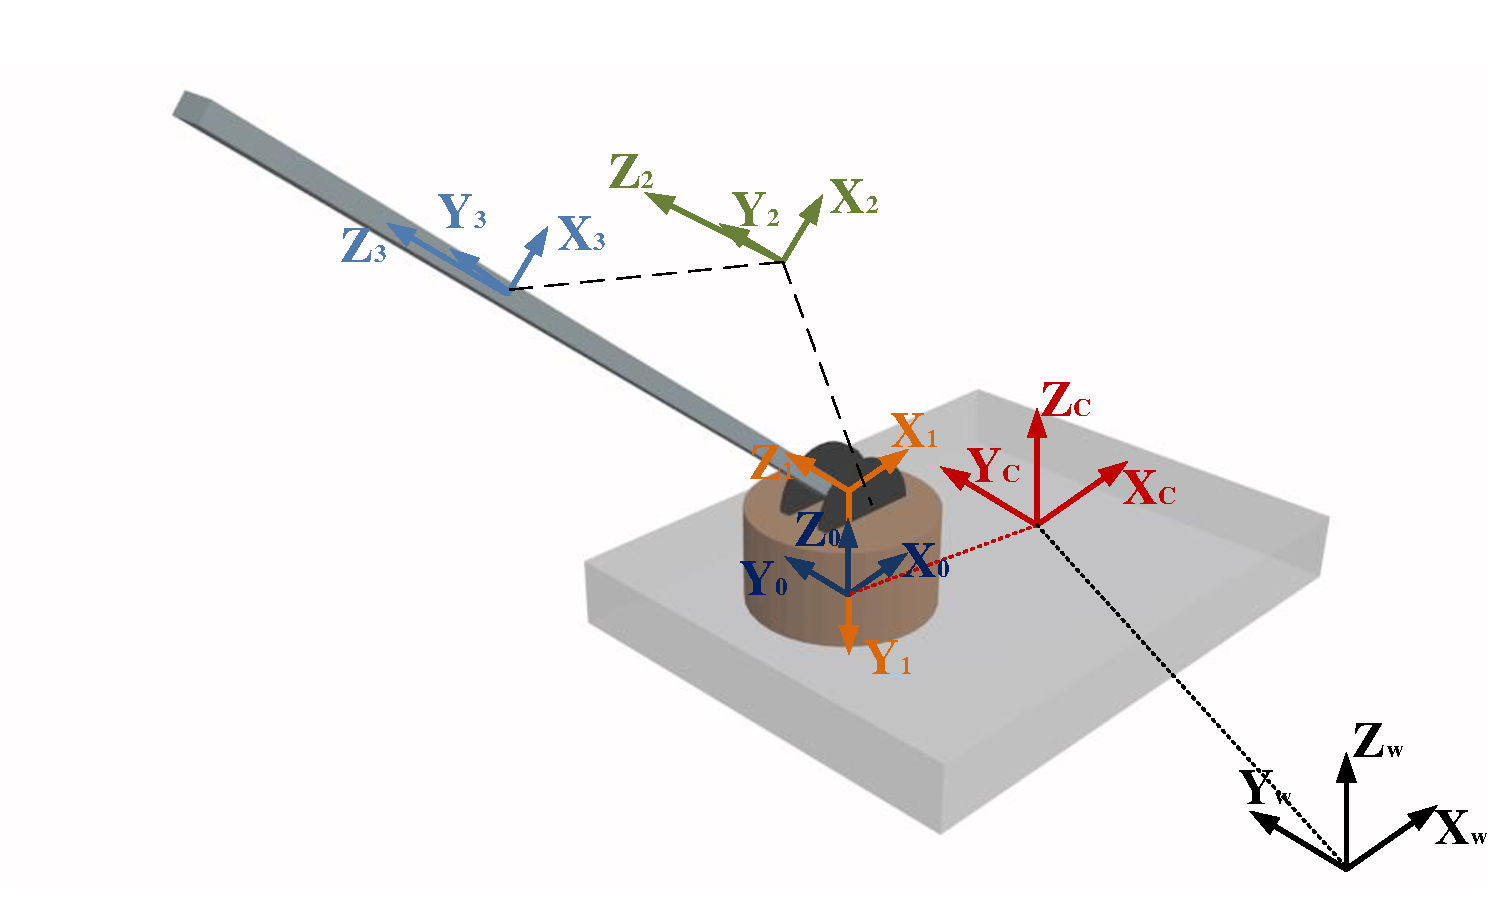
\includegraphics[width=85mm]{./pictures/RobinRepic.pdf}
	\caption{Robin Tail kinematic chain model}
	\label{fig:rmax}
\end{figure}

Equations \eqref{eq:DCH_matrix} show the full complexity of \eqref{eq:NEGeneral} even for a particular case when the quadruped body is at rest. Therefore it is clear, that an analytical solution to the problem of dynamic stabilization through tail motion is not a straight forward process. Instead, we propose using a tail to compensate the imperfections in quadruped construction. Positioning the tail at the right pose, it is possible to shift the balance of the robot and make it symmetric. 
\subsubsection{Tail inertia tensor}
In Fig. \ref{fig:rmoment}, a tail with its ${L_T}$ coordinate system, placed in its center of mass is depicted. Upon introducing the tail as a new body  part in the quadruped construction, the overall center of mass will change accordingly:
\begin{equation}\label{eq:CMrobotAndTail}
\vec{\textbf{r}_{CM}}=\frac{\sum_{i=1}^{4}m_i\vec{\textbf{r}}_i+m_T\vec{\textbf{p}}_T}{\sum_{i=1}^{4}m_i+m_T}= \frac{\Delta\vec{\textbf{r}_{CMB}}+\mu\cdot\vec{\textbf{r}_{CMT}}}{1+\mu}
\end{equation}


In the previous equation we introduced the mass ratio $\mu=\frac{m_T}{\sum_{i=1}^{4}m_i}$ and $\Delta\vec{\textbf{r}_{CM}}$ as the center of mass of the robot without the tail, from equation (\ref{eq:CMrobot}). If we are to keep the center of mass in the construction center of the robot (i.e. $\vec{\textbf{r}_{CM}}=0$), then the following condition has to be met:
\begin{equation}\label{eq:CMzeroing}
\begin{bmatrix}
\Delta \textsc{x}_{cm}\\ 
\Delta \textsc{y}_{cm}\\ 
\Delta \textsc{z}_{cm}
\end{bmatrix}+
\frac{\mu q_3}{2}\begin{bmatrix}
C_1S_2\\ 
S_1S_2\\ 
C_2
\end{bmatrix}=0
\end{equation}
that is to say, that the numerator in (\ref{eq:CMrobotAndTail}) has to be zero. Given that in (\ref{eq:CMzeroing}) there exist only two variables, $q_1$ and $q_2$ respectively, one can eliminate only two components of the center of mass displacement vector $\Delta \vec{\textbf{r}_{CM}}$. Under a reasonable assumption that $\bar{T}\gg \bar{S}$, it follows from the applied torque equation (\ref{eq:Torques}) that for a stable jump one needs to successfully eliminate $x$ and $y$ components of the center of mass displacement vector. This hypothesis is reasonable because in most cases the forward motion is slow compared to vertical jumping, and additionally in z direction one needs to overcome the gravity acceleration $g$. Combining these two assumptions makes the $\bar{T}$ by the order of magnitude larger than $\bar{S}$.

From a strict mathematical point of view, the necessary condition for (\ref{eq:CMzeroing}) to have a solution is:
\begin{equation}\label{eq:CMcondition}
\frac{\mu q_3}{2}\geq \textup{MAX}\left \{ \left | \Delta \textsc{x}_{CM} \right |, \left | \Delta \textsc{y}_{CM} \right |,\left | \Delta \textsc{z}_{CM} \right |\right \}
\end{equation}
When the condtion (\ref{eq:CMcondition}) is met, the analytical solution to equation (\ref{eq:CMzeroing}) can easily be derived:
\begin{gather}\label{eq:CMsolution1}
q_1=atan2\left({\Delta \textsc{y}_{CM}},\, {\Delta \textsc{x}_{CM}}\right)\\
q_2=asin\left(\frac{2\sqrt{{\Delta \textsc{x}_{CM}}^2+{\Delta \textsc{y}_{CM}}^2}}{\mu q_3} \right)\label{eq:CMsolution2}
\end{gather}
Moving the tail joints $q_1$ and $q_2$ to the values calculated with \eqref{eq:CMsolution1} and \eqref{eq:CMsolution2} respectively, balances the quadruped. On the other hand, repositioning the tail changes the overall inertia tensor. This change in the overall inertia can be calculated using the Parallel axis theorem and basic rotation matrices. We start by writing the tail inertia tensor, which, due to the approximation that the tail is infitesimal thin, can be simplified. Written in $L_T$ frame, the tail moment of inertia is:
\begin{equation}\label{eq:JT_LT}
\textbf{J}_T=\textbf{J}_3=\frac{{q_3}^2 m_3}{12}\left(
\begin{array}{ccc}
 1 & 0 & 0 \\
 0 & 1 & 0 \\
 0 & 0 & 0
\end{array}
\right)
\end{equation}
However, in order to write \eqref{eq:JT_LT} in the body coordinate system $L_B$ it needs to be rotated first. After that, the Parallel axis theorem is applied, yielding the equation for the tensor of inertia $J_T$ of the tail. 
\begin{equation}
\begin{aligned}
\scriptsize
{\textbf{J}_T}^*={\textbf{R}_0^3}^T\textbf{J}_T\textbf{R}_0^3+\\+m_T\begin{bmatrix}
{cm_y^T}^2 +{cm_z^T}^2& {cm_x^T}{cm_y^T}& {cm_x^T}{cm_z^T} \\ 
-{cm_x^T}{cm_y^T} & {cm_x^T}^2+{cm_z^T}^2 & {cm_y^T}{cm_z^T}\\ 
-{cm_x^T}{cm_z^T} & -{cm_y^T}{cm_z^T} & {cm_x^T}^2+{cm_y^T}^2
\end{bmatrix}
\normalsize
\end{aligned}
\end{equation}
with $\textbf{R}_0^3$ as a rotation part of transformation matrix \eqref{eq:T03}. Finally, the total moment of inertia is then a sum of the body moment of inertia $\textbf{J}_B$ and the tail moment of inertia $\textbf{J}_T^*$, both written in the body coordinate system.
\begin{equation*}
\textbf{J}_{tot}=\textbf{J}_B+\textbf{J}_T^*
\end{equation*}
